\chapter{Fundamentals-Theory for this approach to reach 5G}
In the following some fundamentals are described shortly.
\section{Concept of Software-defined radio}
The concept of software-defined radio is adapted to deal with the old problems of mobile communication. The idea is to bring the digital domain as close as possible to the RFFE. The reason is digital filtering, data processing is more efficient, easier, less complex, has less cost, and so on. The main problem of this approach is the energy consumption based on an inefficient ADC/DAC. However the concept is very helpful for future designs of an digital front end. The Software-defined radio has the advantage, that it is adaptiv for future software changes. the hardware is still the same, only the firmware has to be upgraded. broad spectrum of signal can be received with this architecture. from nearly DC to 2 GHz. For future mobile communication standards, the frequency range has to deal with frequencies beyond 2 GHz up to 6 GHz. Nowadays IEEE802.11ac standard is located at 5GHz. Based on this concept a digital-analog converter is designed to deal with a higher bandwith than other devices nowadays. The DAC is used in the transmission path of the design.
\section{One possible approach based on SDR: The Riemann Pump}
\subsection{Idea of the concept}
The Riemann Pump, named after the mathematician Riemann, who founded the Riemann Integral, is a special charge pump. This device can convert digital into analog signals based on the concept of a charge pump. Therefore the Riemann Pump is a DAC with a high bandwidth to deal with future standards of mobile communication.

\begin{figure}[ht]
	\centering
  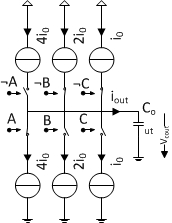
\includegraphics[width=0.5\textwidth]{RiemannPumpConcept.png}
	\caption{Concept of the Riemann Pump with Voltage Sources}
	\label{RiemannPumpConcept}
\end{figure}

 The working principle is to
integrate a current into a capacitive load, this integration is based on Riemann Integral, where the name come from. This integration converts the current into a voltage. This output voltage can be applied to the input of a power amp and then to the antenna to propagate it. The current, which charges the capacitive input of the power amp, is controlled by a digital code. A fixed set of slopes, represents the different current sources. A desired signal in the time-domain is generated with MatLab. This signal can consist of many different signals (different carriers and modulation types). This signal is sampled with the given set of slopes. The minimization of the error leads to the Riemann Code. With this Riemann Code (digital) the driver circuit is controlled. This leads to an analog signal formed by the digital input signal. 
\subsection{implementation of the idea - realisation}
The first approach of designing a Riemann Pump was with a concept of a Push-Pull stage. This push-pull stage should charge a capacitive load at the output, which is the same as a normal charge pump. Push-pull stages complementary switch a high- and lowside transistor as in a charge pump. This was one possible approach. Concept of Maksimovic. 
\subsection{challenges to review - problems}
Same realisation problems, difficulties: Problem of BANDWIDTH, Vpp of control signal (5V pp for GaN transistors), high side driver, no complementary transistors available in III-V technology, low loss driver, high speed driver, digital control driver, too high energy consumption (stability???)